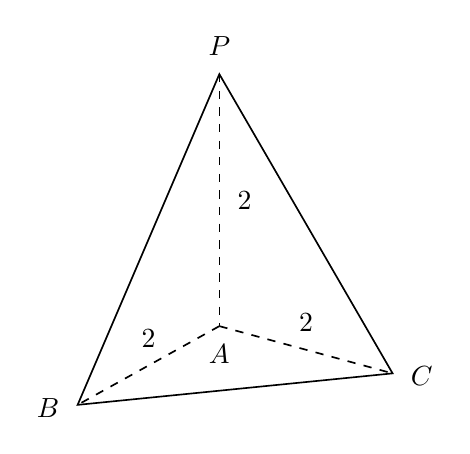
\begin{tikzpicture}[x=2cm,y=2cm,font=\normalsize,line width=.6pt]
\coordinate (P) at (0.0000000000,1.6000000000);
\coordinate (A) at (0,0);
\coordinate (B) at (-0.9,-0.5);
\coordinate (C) at (1.1,-0.3);
% three mutually perpendicular edges at A
\draw[dashed] (P) -- (A);
\draw[dashed] (A) -- (B);
\draw[dashed] (A) -- (C);
% outer faces
\draw[solid] (P) -- (B) -- (C) -- cycle;
\node[above,yshift=3pt] at (P) {$P$};
\node[below=3pt] at (A) {$A$};
\node[left,xshift=-3pt,yshift=-1pt] at (B) {$B$};
\node[right,xshift=3pt,yshift=-1pt] at (C) {$C$};
% edge-length labels placed on free side of each edge
\node[right=3pt] at (0,0.8) {$2$};
\node[above=3pt] at (-0.45,-0.25) {$2$};
\node[above=3pt] at (0.55,-0.15) {$2$};
\end{tikzpicture}
